\documentclass[11pt,aspectratio=169]{beamer}
\usepackage[utf8]{inputenc}
\usepackage[T1]{fontenc}
\usepackage{lmodern}
\usepackage{amsmath}
\usepackage{amsfonts}
\usepackage{amssymb}
\usepackage{graphicx}
\usepackage{tikz}
\usepackage{xspace}
\usepackage{hyperref}
\usepackage{xcolor}
\usetheme{Singapore}

\usepackage{environ}
\makeatletter
\newsavebox{\measure@tikzpicture}
\NewEnviron{scaletikzpicturetowidth}[1]{%
	\def\tikz@width{#1}%
	\def\tikzscale{1}\begin{lrbox}{\measure@tikzpicture}%
		\BODY
	\end{lrbox}%
	\pgfmathparse{#1/\wd\measure@tikzpicture}%
	\edef\tikzscale{\pgfmathresult}%
	\BODY
}

\definecolor{B}{RGB}{200,37,6}
\definecolor{D}{RGB}{3,101,192}

\begin{document}
	\author{Quan Gan}
	\title{Recommender Systems and DGL}
	%\subtitle{}
	%\logo{}
	\institute{AWS Shanghai AI Lab}
	%\date{}
	%\subject{}
	%\setbeamercovered{transparent}
	%\setbeamertemplate{navigation symbols}{}
	\begin{frame}[plain]
		\maketitle
	\end{frame}

	\begin{frame}
		\frametitle{Why Recommendation}
		\only<2>{\begin{center}
			\centering
			\Huge \bf We don't want our customers to think (hard).
		\end{center}}
		\only<3-4>{
			\begin{center}
				\centering
				Good relevant recommendations make the customers adhere to us.
				
				\only<3>{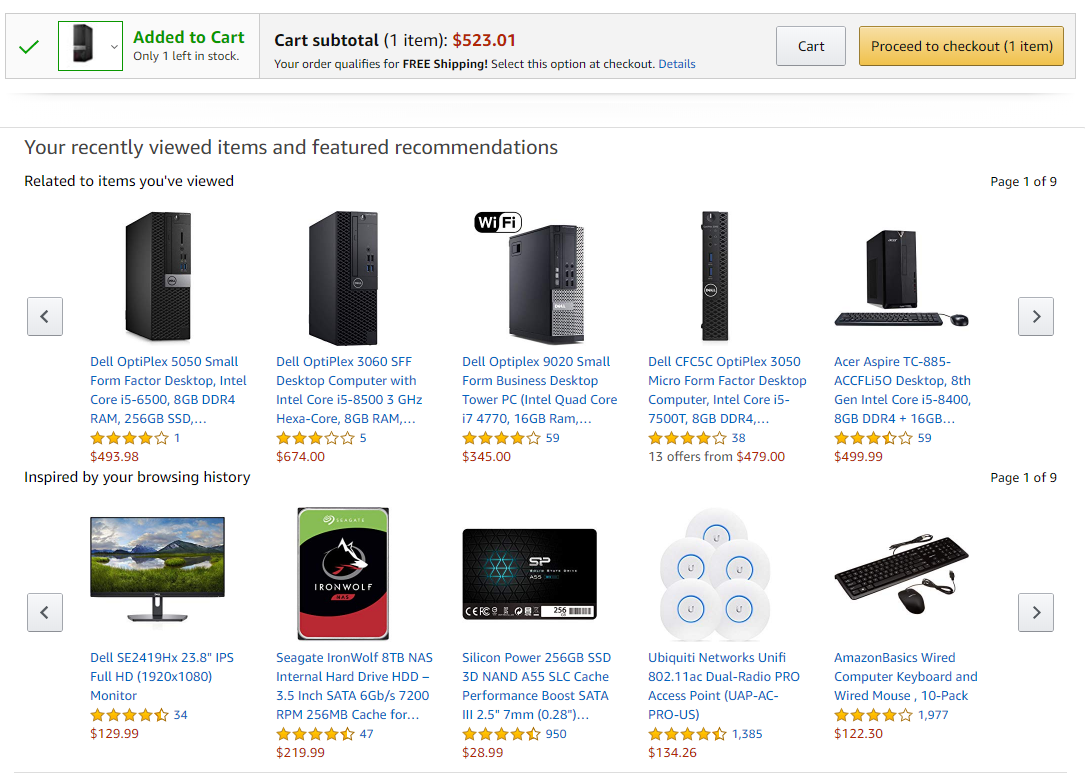
\includegraphics[width=0.8\textwidth]{images/good-recommendation2.png}
				}
				\only<4>{				
\includegraphics[width=0.8\textwidth]{images/good-recommendation.png}}
			\end{center}
		}
	\end{frame}
	
	\begin{frame}
		\frametitle{Recommender System: Problem Statement}
		\begin{center}
			\centering
			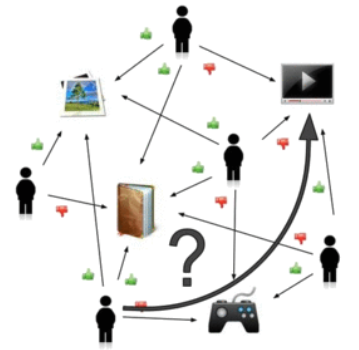
\includegraphics[height=0.7\textheight]{images/cf-stage1.png}
			
			{\tiny Image source: Wikipedia}
		\end{center}
	\end{frame}
	
	\begin{frame}
		\frametitle{Collaborative Filtering}
		\begin{columns}
			\begin{column}{0.3\textwidth}
				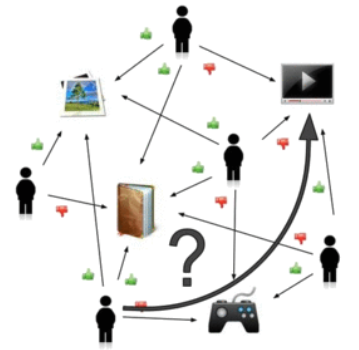
\includegraphics[width=\textwidth]{images/cf-stage1.png}
			\end{column}\pause
			\begin{column}{0.05\textwidth}
				\begin{scaletikzpicturetowidth}{\textwidth}
					\begin{tikzpicture}[scale=\tikzscale]
					\draw [->] (0, 0) -- (0.05, 0);
					\end{tikzpicture}
				\end{scaletikzpicturetowidth}
			\end{column}
			\begin{column}{0.3\textwidth}
				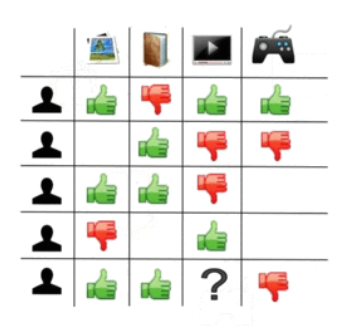
\includegraphics[width=\textwidth]{images/cf-stage2.png}
			\end{column}\pause
			\begin{column}{0.05\textwidth}
				\begin{scaletikzpicturetowidth}{\textwidth}
					\begin{tikzpicture}[scale=\tikzscale]
					\draw [->] (0, 0) -- (0.05, 0);
					\end{tikzpicture}
				\end{scaletikzpicturetowidth}
			\end{column}
			\begin{column}{0.3\textwidth}
				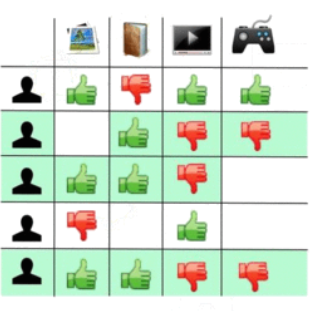
\includegraphics[width=\textwidth]{images/cf-stage3.png}
			\end{column}
		\end{columns}
		\note{Interactions can be inferred by looking at similar users/items.  Users/items are similar if they share some interaction pattern.}
		\begin{center}
			\centering
			{\tiny Image source: Wikipedia}
		\end{center}
	\end{frame}

	\begin{frame}
		\frametitle{Collaborative Filtering: Classical Methods}
		\begin{columns}
			\begin{column}{0.5\textwidth}
				\begin{itemize}
					\item \textbf{User-based}: Infer how a user $i$ would act to an item $j$ by looking at how users that have similar interactions to user $i$ acted to item $j$.
					\begin{itemize}
						\item<2-> We have millions of customers.
						\item<3> User profiles change constantly and quickly, requiring frequent rebuilds (which are expensive already).
						\note[item]{Build complexity is $O(U^2I)$}
					\end{itemize}
				\end{itemize}
			\end{column}
			\begin{column}{0.5\textwidth}
				\begin{center}
					\centering
					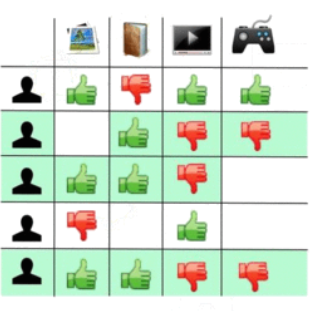
\includegraphics[width=\textwidth]{images/cf-stage3.png}
				\end{center}
			\end{column}
		\end{columns}
	\end{frame}

	\begin{frame}
		\frametitle{Collaborative Filtering: Classical Methods}
		\begin{columns}
			\begin{column}{0.5\textwidth}
				\begin{itemize}
					\item \textbf{\alert<1>{Item}-based}: Infer how a user $i$ would act to an item $j$ by looking at how \alert<1>{items} that have similar interactions to \alert<1>{item $j$} were being acted by \alert<1>{user $i$}.
					\begin{itemize}
						\item Amazon used to have fewer items than users.
						\item<2-> Now we also have millions of items.
						\note[item]{Build complexity is $O(I^2U)$}
					\end{itemize}
				\end{itemize}
			\end{column}
			\begin{column}{0.5\textwidth}
				\begin{center}
					\centering
					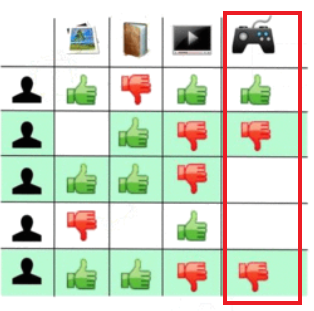
\includegraphics[width=\textwidth]{images/cf-stage3-alter.png}
				\end{center}
			\end{column}
		\end{columns}
	\end{frame}

	\begin{frame}
		\frametitle{Machine Learning Kicks In}
		\begin{columns}
			\begin{column}{0.5\textwidth}
				\begin{center}
					\centering
					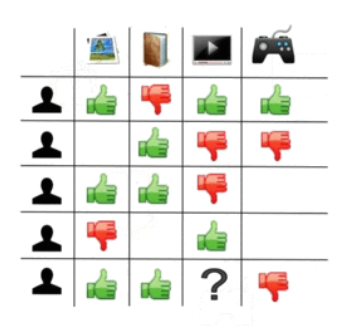
\includegraphics[width=\textwidth]{images/cf-stage2.png}
					
					We were "representing" users and items with the items/users that had interactions with them.
				\end{center}
			\end{column}\pause
			\begin{column}{0.5\textwidth}
				\begin{center}
					\centering
					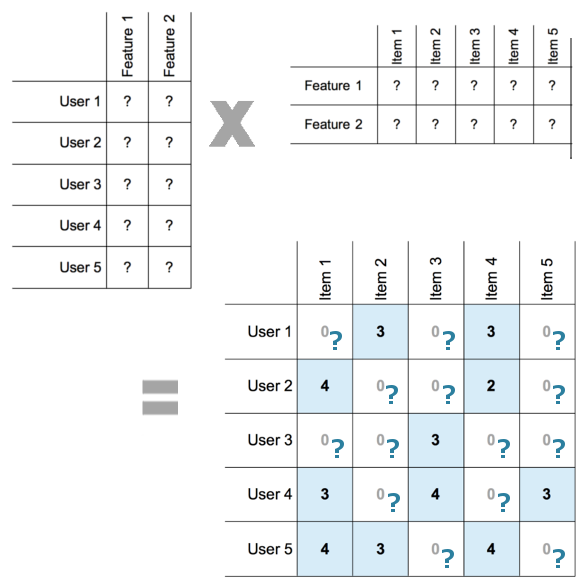
\includegraphics[width=\textwidth]{images/matrix_factorization.png}
					
					{\tiny Source: \href{https://katbailey.github.io/post/matrix-factorization-with-tensorflow/}{\color{blue} Kat Bailey}}
					
					Can we represent users and items as a set of features?
				\end{center}
			\end{column}
		\end{columns}
	\end{frame}

	\begin{frame}
		\frametitle{\only<-3>{Latent Factor Model}\only<4->{Matrix Factorization (Explicit Feedback)}}
		\begin{columns}
			\begin{column}{0.6\textwidth}
				\begin{itemize}
					\item<1-> An item can be described with a \only<1-3>{set of features (e.g. how sweet some food is).}%
					\only<4->{\alert<4>{vector $v_j$}.}
					\item<2-> A user can be described with \only<1-4>{preferences of the same set of features (e.g. how much a user likes sweet food).}%
					\only<5->{\alert<5>{another vector $u_i$}}
					\item<3-> The \only<1-5>{interaction}%
					\only<6->{\alert<6>{rating on item $j$ by user $i$}.}
					is defined by \only<1-5>{how well the item features match the user preferences.}%
					\only<6->{\alert<6>{$u_i^\top v_j$}.}
					\item<7-> \alert<7>{We minimize
					$$
					\begin{gathered}
					\sum_{
						\only<1-9>{i,j}\only<10>{\alert{(i, j) \in \mathcal{B}}}
					}\left(r_{i,j} - \left( u_i^\top v_j
					\only<8->{\alert<8>{+ b_{u_i} + b_{v_j}}}\right) \right)^2 \\
					\only<9->{\alert<9>{+ \alpha\left(
							\left\lVert U \right\rVert_F^2 + 
							\left\lVert V \right\rVert_F^2
							\right)}}
					\end{gathered}
					$$}
				\end{itemize}
			\end{column}
			\begin{column}{0.4\textwidth}
				\begin{center}
					\centering
					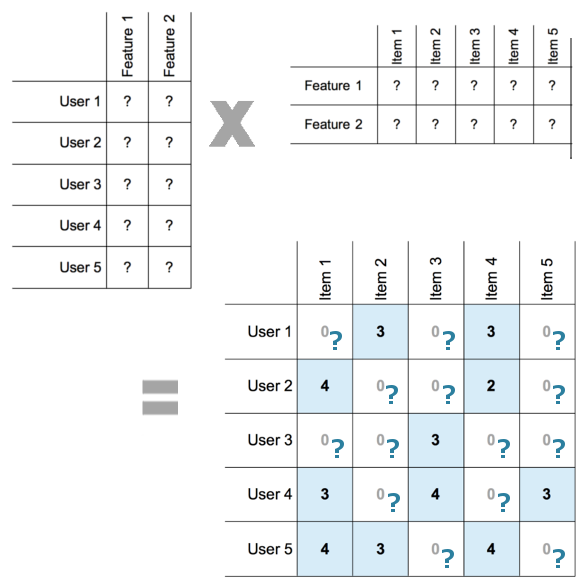
\includegraphics[width=\textwidth]{images/matrix_factorization.png}
					
					{\tiny Source: \href{https://katbailey.github.io/post/matrix-factorization-with-tensorflow/}{\color{blue} Kat Bailey}}
				\end{center}
			\end{column}
		\end{columns}
	\end{frame}

	\begin{frame}
		\frametitle{What if we don't have ratings?}
		\begin{columns}
			\begin{column}{0.5\textwidth}
				\begin{center}
					\centering
					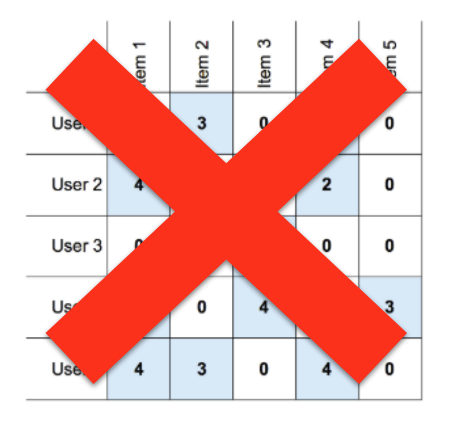
\includegraphics[width=\textwidth]{images/no-rating.png}
				\end{center}
			\end{column}
			\begin{column}{0.5\textwidth}
				\begin{center}
					\centering
					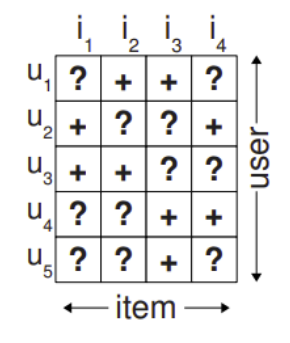
\includegraphics[width=\textwidth]{images/implicit.png}
					
					{\tiny Source: \textit{BPR: Bayesian Personalized Ranking from Implicit Feedback}, Rendle et al. 2012}
				\end{center}
			\end{column}
		\end{columns}
	\end{frame}

	\begin{frame}
		\frametitle{Matrix Factorization (Implicit Feedback)}
		\begin{columns}
			\begin{column}{0.6\textwidth}
				\begin{itemize}
					\item<1-> For a given user $i$, an item being interacted $j$ should have a higher score than another item $k$ which was never being interacted.
					\item<2-> We maximize
					$$
					\sum_{i,j,k\in I \backslash I_{u_i}}
					\log \dfrac{1}{1 + \exp\left(u_i^\top v_k - u_i^\top v_j\right)}
					$$
					\item<3-> We usually \emph{sample} one or multiple $k$ when computing gradients (\textbf{negative sampling}).
					\begin{itemize}
						\item Commonly uniformly, but adaptive sampling often helps.
					\end{itemize}
				\end{itemize}
			\end{column}
			\begin{column}{0.4\textwidth}
				\begin{center}
					\centering
					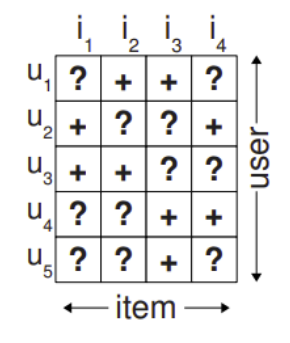
\includegraphics[width=\textwidth]{images/implicit.png}
					
					{\tiny Source: \textit{BPR: Bayesian Personalized Ranking from Implicit Feedback}, Rendle et al. 2012}
				\end{center}
			\end{column}
		\end{columns}
	\end{frame}

	\begin{frame}
		\frametitle{Other Meaningful Aspects to Consider}
		\begin{itemize}
			\item \textbf{Cold-start}: What if we have \textit{new} users and items coming in, with few to no historical interactions? \pause
			\item \textbf{Bias correction}: The training dataset usually comes from the result of a \textit{previous recommender system}.  How to mitigate the bias? \pause
			\item \textbf{Diversity}: Always recommending the same items (or even the same kind of item) to a user would make him/her feel \textit{bored}. \pause
			\item \textbf{Fraud}: How to detect and deal with fabricated explicit feedbacks (e.g. fake ratings and reviews)?
		\end{itemize}
	\end{frame}

	\begin{frame}
		\frametitle{Extensions of Matrix Factorization}
		\begin{itemize}
			\item The score function of vanilla MF: $u_i^\top v_j$ where user and item representations are static and independent of each other (fixing the model).
			\item RNN To integrate user history, $u_i = f(v_{u, 1}, v_{u, 2}, \cdots, v_{u, n})$
			\begin{itemize}
				\item The user representation now depends on his/her previously interacted items.
			\end{itemize}
			\item Graph-based models to integrate neighboring items/users (in the next slide).
			\begin{itemize}
				\item The user representation could also depend on behaviors of other users/items.
			\end{itemize}
			\item Can combine with content-based recommendation (i.e. with user and item features).
			\item Can combine both explicit and implicit feedbacks.
		\end{itemize}
	\end{frame}

	\begin{frame}
		\frametitle{Extensions of Matrix Factorization \tiny (with Graph-based Models)}
		\begin{itemize}
			\item Graph Convolutional Networks on an item copurchase graph
			\begin{itemize}
				\item When new interactions are added, the copurchase graph and the item representation would also change as well.
				\item GCN can also be replaced with other models such as GraphSAGE or PinSAGE (\textit{Hierarchical Temporal Convolutional Networks for Dynamic Recommender Systems}, You et al., 2019)
			\end{itemize}
			\item GCN on the user-item bipartite graph itself
			\begin{itemize}
				\item With one layer, becomes GCMC (van den Berg et al., 2017)
				\item With neighbor sampling, becomes GraphSAGE.
				\item Latest work include STAR-GCN (Zhang et al., 2019) which also deal with cold start problems.
			\end{itemize}
		\end{itemize}
	\end{frame}

	\begin{frame}
		\frametitle{Learning Item Representations with GCN}
		\begin{center}
			\centering
			\includegraphics[width=0.7\textwidth]{images/gcn.png}
			
			{\tiny Source: \textit{Graph Convolutional Neural Networks for Web-Scale Recommender Systems}, Ying et al. 2018}
		\end{center}
		\begin{itemize}
			\item<1-> The graph is a copurchase graph.
			\item<2-> Item features can be projected before GCN.
			\item<3-> During inference, when new copurchases/items appear, we can just recompute the embeddings on the new graph with trained parameters.
		\end{itemize}
	\end{frame}

	\begin{frame}
		\frametitle{Learning Item Representations with GCN}
		\begin{center}
			\centering
			\includegraphics[width=0.7\textwidth]{images/graphsage.png}
		\end{center}
		\begin{itemize}
			\item<1-> GraphSAGE - neighbor sampling
			\item<2-> PinSAGE - Neighbors determined by "top-K most frequent nodes visited by random walk with restarts"
			\begin{itemize}
				\item<3-> In the example: if $K=2$, then \textcolor{B}{B} could also be a neighbor of \textcolor{D}{D}.
				\item<4-> For concrete details of the random walk algorithm, please refer to \textit{Pixie: A System for Recommending 3+ Billion Items to 200+ Million Users in Real-Time}, Eksombatchai et al., 2017
			\end{itemize}
		\end{itemize}
	\end{frame}

	\begin{frame}
		\frametitle{Learning Both User and Item Representations with GCMC}
		\begin{center}
			\centering
			\includegraphics[width=0.6\textwidth]{images/bipartite.png}
			
			{\tiny Source: \textit{Graph Convolutional Matrix Completion}, van den Berg et al. 2017}
		\end{center}
			$$
			\begin{gathered}
			\mu_{j \to i, r} = \dfrac{1}{c_{ij}} W_r x_j\\
			h_i = \sigma \left[\mathrm{accum}\left(
			\sum_{j \in \only<1>{\mathcal{N}_{i,1}}\only<2>{\alert{\mathcal{S}(\mathcal{N}_{i,1})}}} \mu_{j \to i, 1},
			\cdots,
			\sum_{j \in \only<1>{\mathcal{N}_{i,R}}\only<2>{\alert{\mathcal{S}(\mathcal{N}_{i,R})}}} \mu_{j \to i, R}
			\right) \right] \\
			u_i = \sigma(W h_i)\\
			p(\hat{M}_{ij}=r) = \mathrm{softmax}(u_i^\top Q_r v_j)
			\end{gathered}
			$$
	\end{frame}

	\begin{frame}
		\frametitle{Learning Both User and Item Representations with Star-GCN}
		\begin{center}
			\centering
			\includegraphics[width=\textwidth]{images/stargcn.png}
		\end{center}
		\begin{itemize}
			\item Vanilla GCMC can't deal with new users/items without features and with a few interactions.
			\item STAR-GCN
			\begin{itemize}
				\item "Mask" the user/item embedding to 0 as if it is new.
				\item Reconstruct the embedding after the forward pass and reconstruction pass.
			\end{itemize}
		\end{itemize}
	\end{frame}

	\begin{frame}
		\begin{center}
			\centering
			\Huge Coding Session
			
			\Large GraphSAGE on bipartite user-item graph.
		\end{center}
	\end{frame}
\end{document}